\documentclass[10pt]{extarticle}
\usepackage[utf8]{inputenc}
\usepackage[fleqn]{amsmath}
\usepackage{lipsum}
\usepackage{xparse}
\usepackage{graphicx,wrapfig}
\usepackage[bottom=1in,top=1in,left=.75in,right=.75in]{geometry}
\usepackage{xcolor}
\usepackage{enumitem}
\usepackage{tabularx}
\usepackage{array}
\usepackage{subcaption}
\usepackage{float}

\DeclareDocumentCommand{\start}{ O{Kevin Shao \& Jeffrey Cheng} m m m }{#1\\#2\\#3\\#4}
\DeclareDocumentCommand{\blank}{}{\textrm{ }}

\title{Multiple Methods of Classification in R:\\ Classifying Handwritten Numbers 0-9\\\textrm{ }\\\large Regression and Machine Learning}
\date{14 May 2018}
\author{Kevin Shao \& Jeffrey Cheng}

\begin{document}
\allowdisplaybreaks
\hbadness=100001
\renewcommand{\labelitemi}{$>$}
\maketitle
\begin{center}

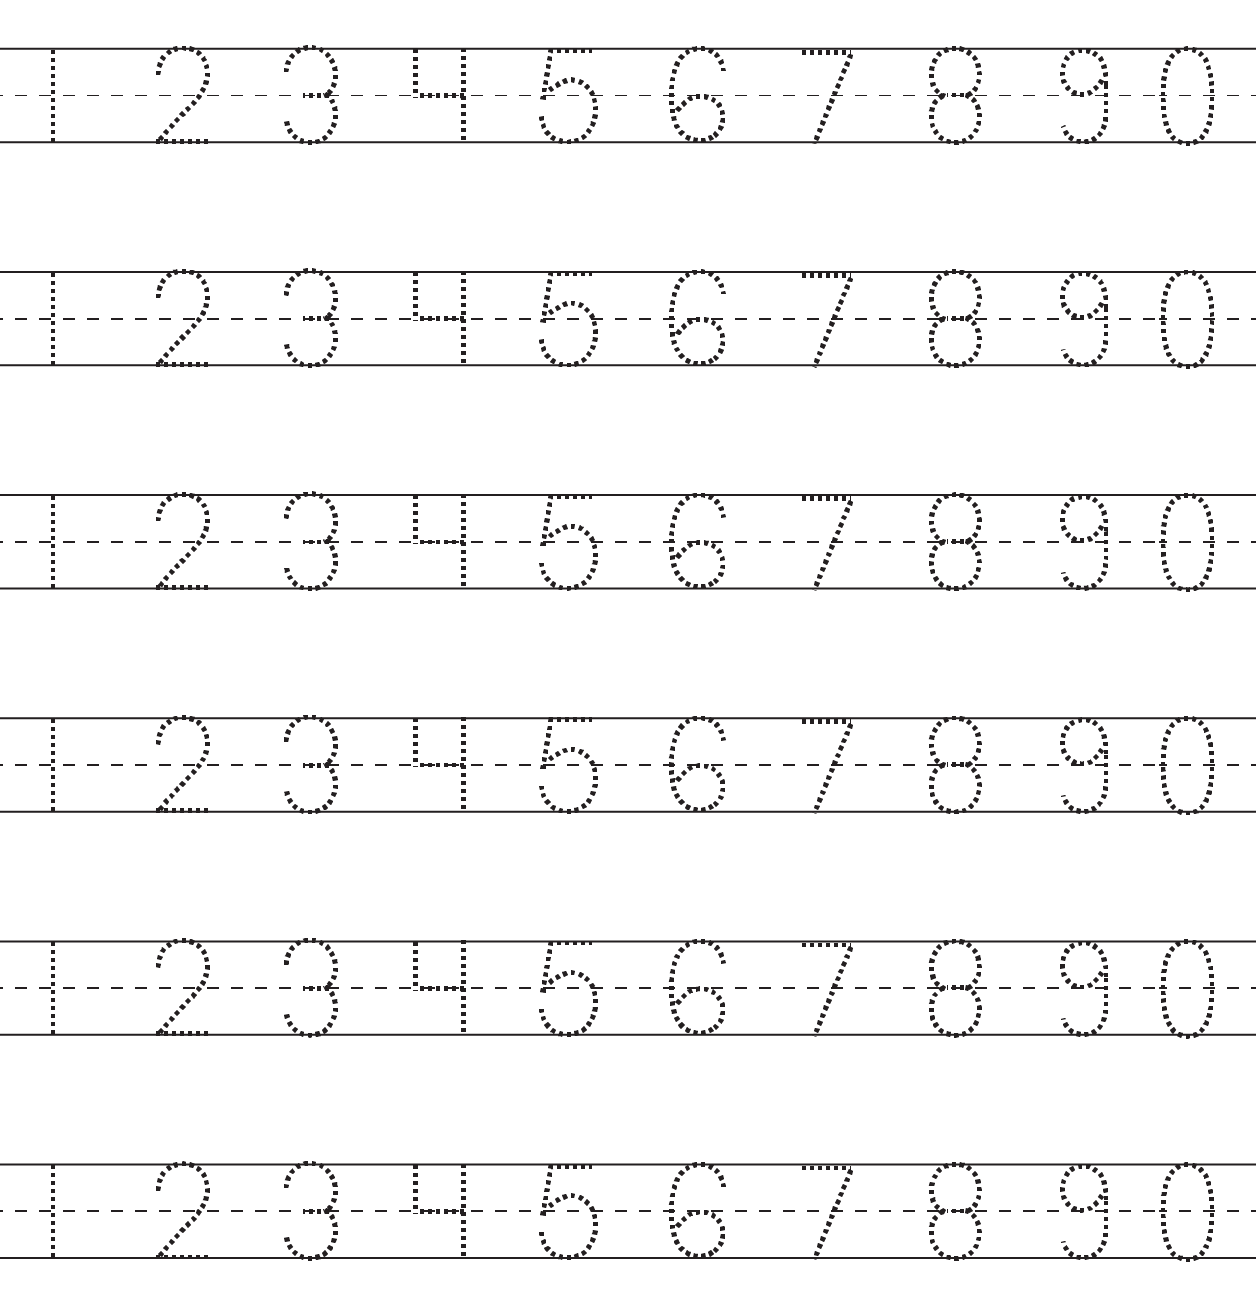
\includegraphics[scale=0.5]{numbers.png}

%\begin{tabular}{c c c}
%	\includegraphics{one.png} & \includegraphics{two.png} & \includegraphics{three.png}\\
%	\includegraphics{four.png} & \includegraphics{five.png} & \includegraphics{six.png}\\
%	\includegraphics{seven.png} & \includegraphics{eight.png} & \includegraphics{nine.png}
%\end{tabular}
\end{center}
\newpage

\section{Abstract}

The MNIST dataset (http://yann.lecun.com/exdb/mnist/) is a classic dataset in the field of computer vision. The task is to classify simple black-and-white images of handwritten digits as its value (0-9). The each input observation comes in the form of 784 (28x28) numbers, ranging from 0-255, indicating the intensity of the color at the pixel (0 is white, 255 is black). There are four files: training images, test images, training labels, and test labels. Each is in the form of a data file. The format is very simple and can be found on the website, so it won't be expanded on here. We used a simple Python script to port the data to a CSV file.
Because the explanatory variables represent individual pixels within different images, it is not really helpful to perform a five number summary. 

\section{Preprocessing}

Aside from porting to CSV format, there was not much general preprocessing to be done. Most of the data processing was specific to each classification method. Our training data set consisted of 59999 observations while our test set had 9999 observations. All observations had 785 columns, the first column begin the true number followed by the rest of the pixel data. An example of each number is shown below:
\begin{center}
	\begin{tabular}{c c c c c c c c c c}
		\includegraphics{zero.png} & \includegraphics{one.png} & \includegraphics{two.png} 
		\includegraphics{three.png} & \includegraphics{four.png} & \includegraphics{five.png} 
		\includegraphics{six.png} &\includegraphics{seven.png} &\includegraphics{eight.png} 
		\includegraphics{nine.png}
	\end{tabular} 
\end{center}
\section{LDA}

There were two main problems when attempting to do LDA on the dataset. Firstly, since the training and test sets are so big, the time it would take R to complete the LDA classification would be substantially long. Thus to counteract this problem, we took a small subset of our training and test sets. Since they were already randomized, there is no need to take a random sample, thus we took the first 2000 observations of the training set and the first 500 observations of the test set.\\\\
The second problem is that some of the pixels remain white through all the images. So, when R attempts to do lda, it indicates that the variables are constant. To counteract this problem, we took the sums of the columns of the dataset, which corresponds to the total grayscale of a specific pixel throughout all 2000 training images. If the sum was greater than an arbitrary number, say 1000, we used the column in our lda. If the sum were less than that arbitrary number, then we removed it from the data set. Using 1000 as our arbitrary number for now, we obtained a test and training error and corresponding confusion matrices.
\begin{center}
	\begin{tabular}{c c}
		Training Error & Test Error\\
		0.041 & 0.246
	\end{tabular}\\
\end{center}
\begin{minipage}{.55\textwidth}
	\begin{center}
	\begin{tabular}{c | c c c c c c c c c c}
		d \textbackslash r&0&1&2&3&4&5&6&7&8&9\\ \hline
		0&186&0&1&0&0&0&0&0&1&0\\
		1&0&214&3&0&1&1&1&6&3&0\\
		2&0&0&187&0&0&1&0&0&0&0\\
		3&1&1&0&185&0&2&0&0&0&0\\
		4&0&0&2&0&203&1&0&1&0&6\\
		5&0&2&0&2&2&171&0&0&1&1\\
		6&1&0&0&0&1&1&199&0&1&0\\
		7&0&0&1&1&0&0&0&210&0&3\\
		8&3&2&3&0&1&2&0&0&165&2\\
		9&0&1&1&3&6&1&0&7&1&198
	\end{tabular}\\
	\bigskip
	Training Set Confusion Matrix
	\end{center}
\end{minipage}
\begin{minipage}{.09\textwidth}
	\quad
\end{minipage}	
\begin{minipage}{.35\textwidth}
The d and the r refer to data and reference. So, the numbers running along the top of the matrix are the true numbers while the numbers along the left are what lda predicts. There are no consistent errors in the data set. The greatest errors come from confusing 4s with 9s, a task not teachers can consistently get right (for all those times that Dr. Brown couldn't read my handwriting).
\end{minipage}\\
\begin{minipage}{.45\textwidth}
	It is interesting how much lower the traing error is than the test error. We thought this was due to the fact that the lda model that we created was still more tailored to the training set we created. If our training set were bigger, the discrepancy between training and test error would decrease. Nonetheless, the both errors we got, were much lower than the 90\% error we would obtain from randomly classifying.
\end{minipage}
\begin{minipage}{.05\textwidth}
	\quad
\end{minipage}
\begin{minipage}{.5\textwidth}
	\begin{center}
	\begin{tabular}{c | c c c c c c c c c c}
		d\textbackslash r & 0 & 1 & 2 & 3 & 4 & 5 & 6 & 7 & 8 & 9\\ \hline
		0&35&0&0&0&1&1&2&0&0&0\\
		1&0&66&6&0&1&1&1&1&1&1\\
		2&1&0&36&2&1&3&4&2&2&0\\
		3&1&0&1&34&1&3&0&1&1&1\\
		4&0&0&2&0&41&1&2&0&4&7\\
		5&3&1&1&5&0&36&2&0&2&2\\
		6&0&0&2&0&1&1&32&0&0&0\\
		7&0&0&2&1&0&0&0&33&2&5\\
		8&1&0&4&1&0&3&0&0&27&1\\
		9&1&0&1&3&9&1&0&11&1&37\\
	\end{tabular}
	\bigskip
	Test Set Confusion Matrix
	\end{center}
\end{minipage}	
We wondered if we could improve upon our error if we changed the arbitrary value of 1000 we initially chose. So, we wrote a function that takes in the value of for which the sum of pixels in the training set needs to be greater than and returns the test and training errors.\\\\\\
\begin{minipage}{.25\textwidth}
	\begin{tabular}{c c c}
		sum & Training & Test\\ \hline
		50&0.0340&0.274\\
		100&0.0340&0.272\\
		150&0.0335&0.264\\
		200&0.0375&0.256\\
		250&0.0345&0.260\\
		300&0.0345&0.258\\
		350&0.0350&0.253\\
		400&0.0350&0.246\\
		450&0.0355&0.248\\
		500&0.0370&0.244
	\end{tabular}
\end{minipage}
\begin{minipage}{.25\textwidth}
	\begin{tabular}{c c c}
		sum & Training & Test\\ \hline
		550&0.0365&0.240\\
		600&0.0390&0.243\\
		650&0.0385&0.245\\
		700&0.0385&0.238\\
		750&0.0395&0.238\\
		800&0.0400&0.242\\
		850&0.0405&0.244\\
		900&0.0410&0.244\\
		950&0.0410&0.244\\
		\textbf{1000}&\textbf{0.0410}&\textbf{0.246}\\
	\end{tabular}
\end{minipage}
\begin{minipage}{.25\textwidth}
	\begin{tabular}{c c c}
		sum & Training & Test\\ \hline
		1050&0.0400&0.240\\
		1100&0.0400&0.244\\
		1150&0.0405&0.246\\
		1200&0.0405&0.242\\
		1250&0.0405&0.232\\
		1300&0.0420&0.236\\
		1350&0.0420&0.232\\
		1400&0.0425&0.236\\
		1450&0.0425&0.236\\
		1500&0.0425&0.238	
	\end{tabular}
\end{minipage}
\begin{minipage}{.25\textwidth}
	\begin{tabular}{c c c}
		sum & Training & Test\\ \hline
		1550&0.0425&0.238\\
		1600&0.0435&0.238\\
		1650&0.0435&0.234\\
		1700&0.0450&0.234\\
		1750&0.0445&0.236\\
		1800&0.0445&0.236\\
		1850&0.0445&0.236\\
		1900&0.0450&0.232\\
		1950&0.0450&0.232\\
		2000&0.0455&0.230
	\end{tabular}
\end{minipage}\\\\\\
The bolded text represents the (sum = 1000) that we initially chose. There is an interesting trend, as sum increases, training error increases while test error decreases. This can be explained by thinking about how sum is related to the number of explanatory variables. As sum increases, the required sum for the total colored pixels increases, thus we are more exclusive in choosing explanatory variables. In essence, as sum increases, the number of explanatory variables decreases. This would explain why a large number of explanatory variables (low sum) has a low training error, the more explanatory variables the better. However, this does not hold true for test error. Since the test set is a whole new dataset, using the more important variables (greater sum) would result in a lower test error, as shown by the data.\\\\
Is there another way to use lda to classify the variables? Since even using the reduced number of variables takes a long time for R to process, we wondered if the total number of colored pixels was related to the true number. After all, some numbers can be written using less pixels (read: ink) than others. Thus, we took a slightly larger training and test set, 10000 and 2500, respectively, and ran lda on the data.\\\\
\begin{minipage}{.45\textwidth}
\begin{center}
\begin{minipage}{.45\textwidth}
	\begin{tabular}{c c}
	number & fill\\ \hline
	0& 194.87712\\
	1&  89.11003\\
	2& 168.83653\\
	3& 165.40174\\
	4& 143.07959
	\end{tabular}
\end{minipage}
\begin{minipage}{.45\textwidth}
	\begin{tabular}{c c}
	number & fill\\ \hline
	5& 149.38631\\
	6& 157.02761\\
	7& 133.80748\\
	8& 173.62288\\
	9& 145.44683
	\end{tabular}
\end{minipage}
\begin{tabular}{c}
	Test Error\\
	0.778
\end{tabular}
\end{center}
\end{minipage}
\begin{minipage}{.6\textwidth}
	\begin{center}
	\begin{tabular}{c | c c c c c c c c c c}
	d\textbackslash r&0&1&2&3&4&5&6&7&8&9\\ \hline
	0&79&1&63&47&25&34&46&10&83&16\\
	1&2&274&17&22&52&15&15&98&6&31\\
	2&8&0&5&2&2&6&1&0&4&2\\
	3&69&0&53&52&32&40&32&17&62&31\\
	4&0&0&0&0&0&0&0&0&0&0\\
	5&0&0&0&0&0&0&0&0&0&0\\
	6&27&2&49&25&31&29&32&19&24&24\\
	7&24&10&85&96&124&88&90&109&59&134\\
	8&6&0&1&1&2&4&1&0&0&2\\
	9&4&0&4&9&7&5&8&3&4&4
	\end{tabular}\\
	\bigskip
	Test Set Confusion Matrix
	\end{center}
	\textrm{ }
\end{minipage}
The test error is so high because the group means shown above are so close to each other. This is also reflected in the confusion matrix, not one observation in the test set was classified as either a 4 or 5. While some numbers, such as one, were consistently correctly classified due to its unique pixel count, there were too many numbers that had a pixel count of around 140, which led to severe misclassification.

\section{QDA} %TODO: OVER HERE

QDA is usually more accurate than LDA, but just requires more resources to run. So, we expected both training and test errors for QDA to be lower than that of LDA. Using QDA also gave several errors we had to fix with preprocessing. Firstly, there was the issue that the number of columns exceeded the minimum number of observations for a class. In order to address this issue, we increased the amount of total observations. Instead of a subset of 2000 like in LDA, we took a subset of 20000. The test set increased accordingly as well to 5000.\\\\
Another issue was that QDA saw that we had too many collinear variables, too many of the variables had zeros. Thus, that number n that we arbitrarily assigned to 1000 in LDA had to increase as well to decrease the number of explanatory variables we had. Even after accounting for the increased sample size, we had to increase n by a factor of 1000, to 1000000 for the QDA to work. Using these new parameters, we got the following values.

\begin{center}
	\begin{tabular}{c c}
		Training Error & Test Error\\
		0.03315 & 0.102
	\end{tabular}\\
\end{center}
\begin{minipage}{.7\textwidth}
	\begin{center}
	\begin{tabular}{c | c c c c c c c c c c}
		d \textbackslash r&0&1&2&3&4&5&6&7&8&9\\ \hline
		0&1973&0&4&3&2&6&5&1&0&11\\
		1&0&2148&1&2&0&0&4&0&3&2\\
		2&7&31&1880&18&13&1&1&35&4&10\\
		3&2&7&2&1987&0&5&2&6&8&22\\
		4&0&13&6&1&1896&0&0&19&1&11\\
		5&6&3&0&12&0&1744&22&3&3&0\\
		6&0&0&6&0&4&1&1911&0&0&0\\
		7&1&1&6&6&3&0&0&1983&0&6\\
		8&5&76&24&41&6&15&26&19&1900&37\\
		9&0&2&0&6&21&3&0&27&3&1915
	\end{tabular}\\
	\bigskip 
	Training Set Confusion Matrix
	\end{center}
	\textrm{ }
\end{minipage}
\begin{minipage}{.3\textwidth}
Right off the bat, we can see that both training and test errors are lower than those of LDA, which is good. Interestingly, the most misclassifications are no longer between 4s and 9s, but rather other random numbers such as 1s and 8s that don't appear to have anything in common at first sight.\\\\
\end{minipage}
\begin{minipage}{.35\textwidth}
	Just like in LDA, the test error is slightly greater than training error. However, we increased the number of observations, and the discrepancy became lower, just as we predicted it would. Otherwise, there are no big discrepancies between the test and training sets.
\end{minipage}
\begin{minipage}{.05\textwidth}
	\quad
\end{minipage}
\begin{minipage}{.6\textwidth}
	\begin{center}
	\begin{tabular}{c | c c c c c c c c c c}
		d\textbackslash r & 0 & 1 & 2 & 3 & 4 & 5 & 6 & 7 & 8 & 9\\ \hline
		0&451&0&4&5&0&8&9&1&3&7\\
		1&0&537&1&0&0&0&2&2&0&2\\
		2&3&8&486&12&6&0&7&35&1&7\\
		3&0&3&9&434&0&15&1&6&19&10\\
		4&0&1&5&1&463&0&4&14&1&17\\
		5&1&0&0&14&0&391&12&1&1&1\\
		6&0&0&2&1&4&1&403&0&0&0\\
		7&0&0&1&1&2&1&0&411&0&2\\
		8&5&22&22&30&9&39&24&24&462&22\\
		9&0&0&0&3&16&1&0&17&2&452\\
	\end{tabular}\\
	\bigskip
	Test Set Confusion Matrix
	\end{center}
	\textrm{ }
\end{minipage}	
The further analysis we did with LDA holds true here as well, we just did not feel the need to manually input that many tables again to prove the same point.
\section{KNN}
In contrast with other methods for machine learning, KNN is a form of lazy classification. That is, it defers all computation to the testing phase. In fact, there is no training phase; all the work is done upon testing an image, whereupon the $k$ closest neighbors are computed, and the test image is classified most frequently occurring class. Proximity, in our implementation, is simply $n$-dimensional Euclidian distance.\\\\
For such a large dataset, especially for a manual implementation, it was important to bear in mind the complexity of the computation. Our essential code, the part that actually executes KNN, is as follows. 
\begin{verbatim}
knn <- function (input, k = 7) {
  differences = sweep(arr, 2, input, "-", check.margin = FALSE )
  differences = differences * differences
  distances = rowSums(differences)
  indices = order(distances)[1:k]
  votes = train[indices, 1]
  prediction = strtoi(names(which.max(table(votes))))
  return (prediction)\\\\
}
\end{verbatim}
As input to our function, we take input, a 784 dimensional vector of pixel intensities, along with an optional $k$ value, which defaults to 7 (reducing the chance of ties, as most ambiguous digits are between two possibilities, such as 4 and 9, 3 and 8, etc). \\\\
In the first line of the function, we take advantage of the built-in R "sweep" function. The variable "arr" is a 60000$\times$784 matrix, where the $i$-th row is the 784 dimensional vector representing the pixel intensities of the $i$-th training observation. In essence, the "sweep" function applies a given function, in this case subtraction (hence the "-"), along a given axis, in this case vertically (hence the 2), on each row of a given matrix, in this case "arr", by a given vector, in this case our input. The result, then, is a 60000$\times$784 matrix, where the $i$-th row is the 784 dimensional vector representing the differences in pixel intensities between the $i$-th training observation and the test observation. The next line squares the matrix element-wise, and the following one collapses the matrix into a 60000 dimensional vector by summing each row. With three short lines, then, we have arrived at the squared distance from the test input to each training point. Since the square root function is monotonically increasing and only the order of the distances is relevant, it is unnecessary to take the computationally expensive step of taking the square root. \\\\
Next, we use the R function "order" to sort the distances from least to greatest, and take the first $k$ of them (hence the [1:k]). We then convert it into a table, with "table(votes)", then take the most frequent appearance, with "which.max". After some simple parsing, we return our prediction. \\\\
With this implementation of KNN and choice of $k$, we arrive at a test error rate of 3\%. The confusion matrix is as follows.
\begin{center}
\begin{minipage}{.6\textwidth}
	\begin{center}
	\begin{tabular}{c | c c c c c c c c c c}
	d\textbackslash r&0&1&2&3&4&5&6&7&8&9\\ \hline
	0& 974 & 0 & 11 & 0 & 1 & 5 & 6 & 0 & 6 & 5\\
	1&1&1133&8&3&8&0&3&25&4&6\\
	2& 1 & 2 & 988 & 2 & 0 & 0 & 0 & 3 & 0 & 0\\
	3& 0 & 0 & 2 & 976 & 0 & 8 & 0 & 0 & 11 & 6\\
	4& 0 & 0 & 1 & 1 & 945 & 2 & 3 & 1 & 7 & 8\\
	5& 1 & 0 & 0 & 12 & 0 & 866 & 2 & 0 & 12 & 4\\
	6& 2 & 0 & 2 & 1 & 5 & 4 & 944 & 0 & 1 & 1\\
	7& 1 & 0 & 16 & 7 & 1 & 1 & 0 & 988 & 6 & 11\\
	8& 0 & 0 & 4 & 4 & 1 & 2 & 0 & 0 & 916 & 2\\
	9& 0 & 0 & 0 & 4 & 21 & 4 & 0 & 10 & 5 & 963
	\end{tabular}\\
	\bigskip
	Test Set Confusion Matrix
	\end{center}
	\textrm{ }
\end{minipage}
\end{center}
As is surprisingly human, the principal misclassifications are misclassifying 7's as 1's, 4's as 9's, 2's as 7's and 8's as 3's or 5's. Interestingly, their converses are generally far more accurate. \\\\
The main drawback to KNN is the runtime complexity. After all, even with our vectorized approach (using the sweep method), our algorithm runs with complexity $O(784n)$, which, in this case, translated to taking ~5 seconds to classify a single digit, far inferior to human speeds. 


\section{Random Forest}

We needed to change the names of the variables since randomForest cannot read a string that looks like an integer for some reason. Thus, we just preppended an 'x' before each name. The naming scheme for each variable is simple, they are in the format of "x.a.b" where x is the aforementioned preppended letter, a is the row the pixel corresponds to on the actual image, and b is the column the pixel corresponds to. Completing the random forest classification, we are able to plot the result.\\\\
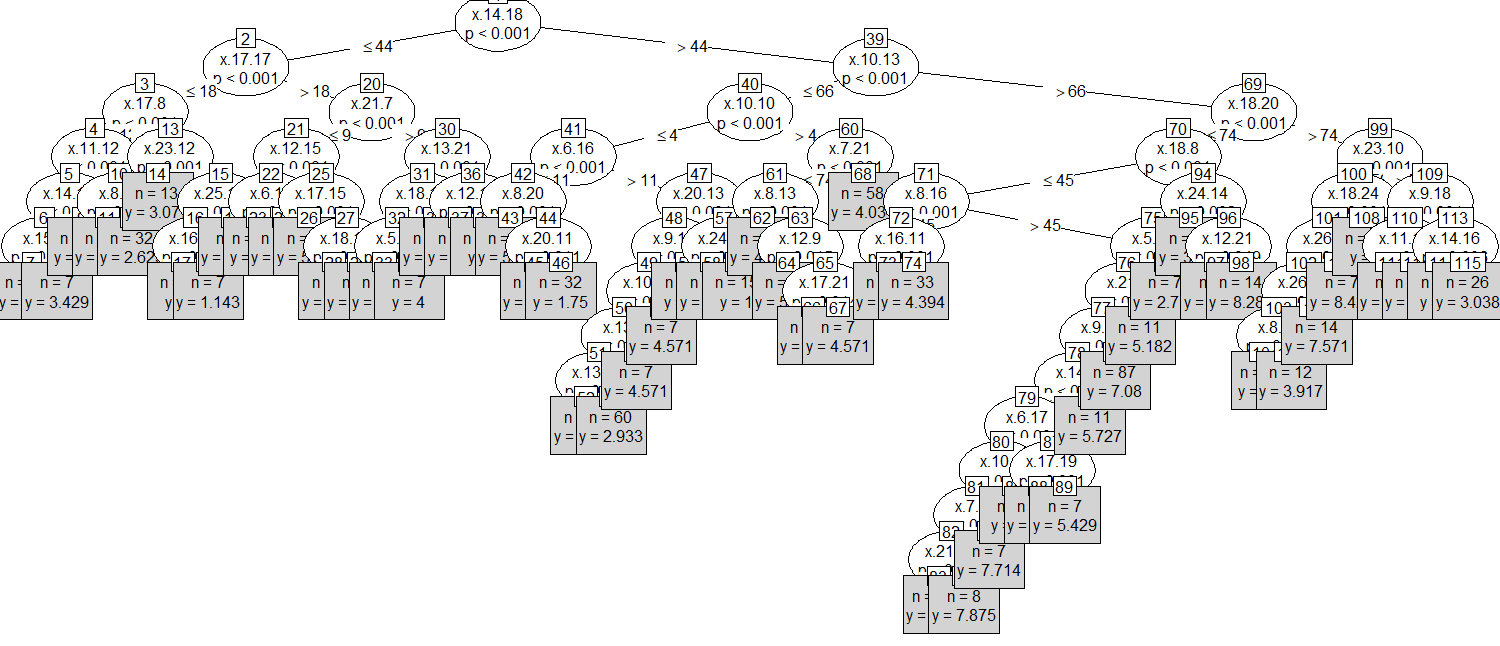
\includegraphics[scale=0.45]{Rplotforest.png}\\\\
The extremely dense formatting of the boxes aside, we only need to look at the topmost split to show why random forest is a terrible way to classify our data. The first split occurs at 14.18, and begins the classification based on the color of that pixel. Essentially, all the splits are performed by looking at the greyscaling of a \textbf{specific} pixel. Even if the training error happened to be low, if each number that was drawn was just shifted one pixel over, then the entire model would fail. The only feasible way for this model to work is to take each image, crop all the whitespace around it, rescale it back to size and give it artificial greyscaling, so the position and size of each image would match the others. However, this is next to impossible, which makes using a different classification method the better approach.\\\\
\begin{minipage}{.55\textwidth}
\begin{center}
\begin{tabular}{c | c c c c c c c c c c}
	 d\textbackslash r&0& 1& 2& 3& 4& 5& 6& 7& 8& 9\\ \hline
	 0&70& 0& 0& 0& 0& 0& 0& 0& 0& 0\\
	 1&65 &154& 0& 0& 0& 0& 1& 0& 0& 1\\
	 2&31&45&64& 3& 0& 0& 1& 2& 0& 1\\
	 3&16&13&83&80& 3& 3& 3& 4& 2& 1\\
	 4& 8& 4&31&74 &102&46&14& 6& 9& 2\\
	 5& 1& 2&14&23&92& 106&75&21&32&10\\
	 6& 0& 1& 5& 7&13&24& 106&54&57&26\\
	 7& 0& 1& 0& 4& 4& 0& 0& 134&49&42\\
	 8& 0& 0& 1& 0& 0& 1& 0& 3&23&65\\
	 9& 0& 0& 0& 0& 0& 0& 0& 0& 0&62
\end{tabular}
\bigskip
Training Set Confusion Matrix
\end{center}
\end{minipage}
\begin{minipage}{.4\textwidth}
Another problem with random forests is that it treated our classes as continuous variables, so we rounded to obtain integer values. This is shown in our confusion matrix, as all the error is from misclassifying numbers that are neighbors numerically, not by shape.
\begin{center}
	\begin{tabular}{c c}
		Training Error & Test Error\\
		0.5495 & 0.9000
	\end{tabular}
\end{center}
\end{minipage}\\
\begin{minipage}{.45\textwidth}
	The test error is 90\%, which is essentially just random classification. This result is consistent with what we predicted above. The training error is surprisingly semi-decent, but still nowhere close to as accurate as other methods above.
\end{minipage}
\begin{minipage}{.05\textwidth}
	\quad
\end{minipage}
\begin{minipage}{.4\textwidth}
\begin{tabular}{c | c c c c c c c c c c}
 d\textbackslash r&0&1&2&3&4&5&6&7&8&9\\ \hline
 0&3&2&6&3&5&1&5&2&3&5\\
 1&5&10&5&13&7&9&2&5&8&7\\
 2&2&6&2&5&6&6&3&5&3&5\\
 3&7&9&10&1&8&3&7&3&6&5\\
 4&6&8&3&6&7&4&4&8&6&9\\
 5&2&7&8&3&3&4&6&2&3&6\\
 6&5&5&8&7&3&10&4&4&4&5\\
 7&7&10&7&4&5&5&8&12&3&7\\
 8&3&5&1&1&3&1&4&4&4&2\\
 9&2&5&5&3&8&7&0&3&0&3
 \end{tabular}
\end{minipage}

\section {Interesting (Mis)classifications}

In this section, we will present interesting cases where KNN, our most accurate classifier, failed to correctly identify the digit. Interestingly, from a human perspective, many of these misclassifications are somewhat understandable.

\begin{table}[H]
\begin{tabular}{c c c}
\begin{subfigure}{0.3\textwidth}\centering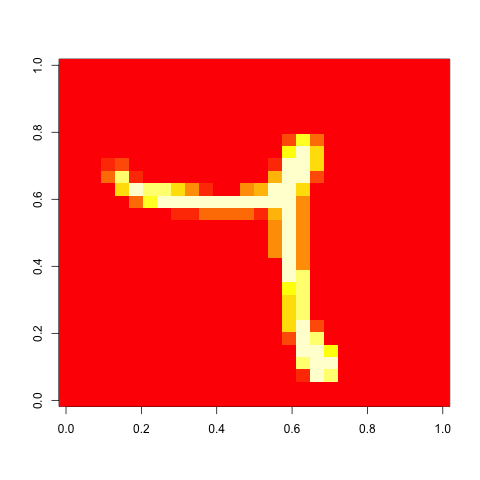
\includegraphics[scale = .25]{../Images/358.png}\caption{Case 358: Predict - 4, True - 7.}\label{fig:taba}\end{subfigure}&
\begin{subfigure}{0.3\textwidth}\centering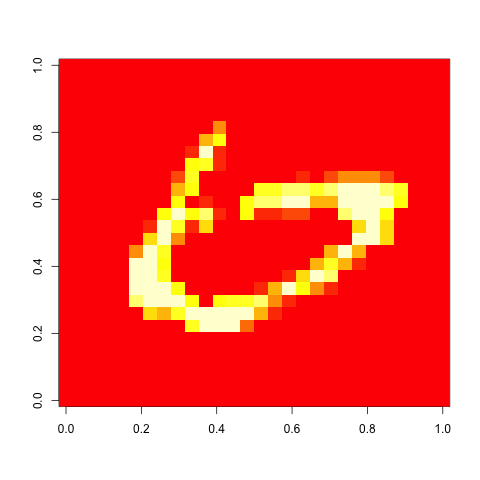
\includegraphics[scale = .25]{../Images/445.png}\caption{Case 445: Predict - 0, True - 6.}\label{fig:taba}\end{subfigure}&
\begin{subfigure}{0.3\textwidth}\centering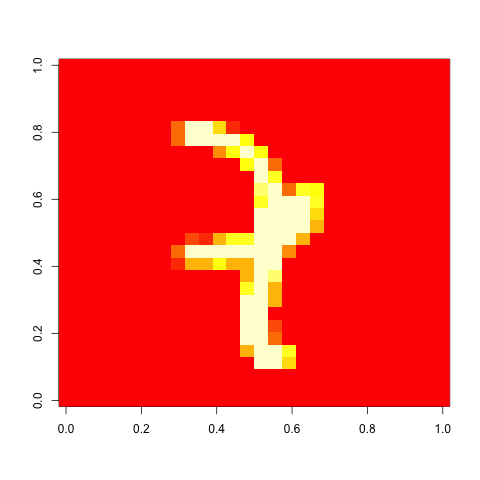
\includegraphics[scale = .25]{../Images/551.png}\caption{Case 551: Predict - 1, True - 7.}\label{fig:taba}\end{subfigure}
\end{tabular}
\end{table}
\newpage
\begin{table}{H}
\begin{tabular}{c c c}
\begin{subfigure}{0.3\textwidth}\centering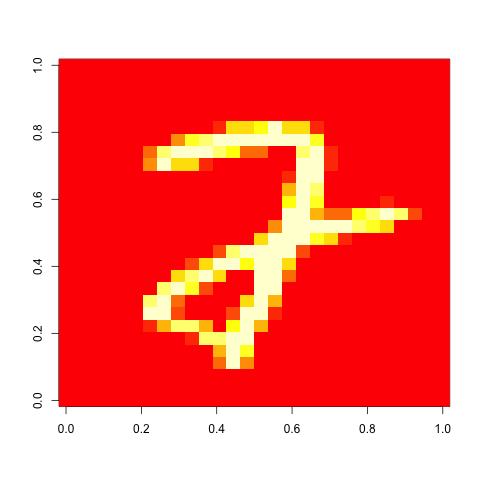
\includegraphics[scale = .25]{../Images/583.png}\caption{Case 583: Predict - 7, True - 2.}\label{fig:taba}\end{subfigure}&
\newline
\begin{subfigure}{0.3\textwidth}\centering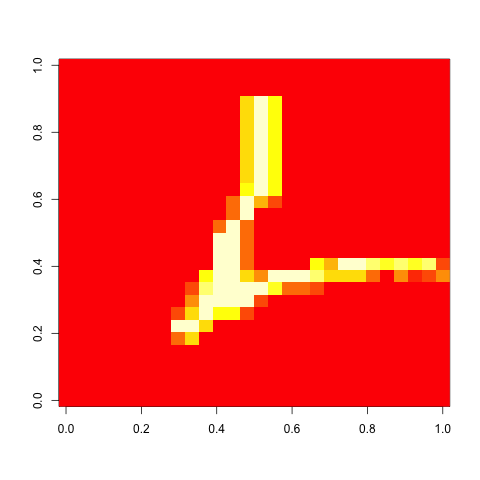
\includegraphics[scale = .25]{../Images/646.png}\caption{Case 646: Predict - 6, True - 2.}\label{fig:taba}\end{subfigure}&
\begin{subfigure}{0.3\textwidth}\centering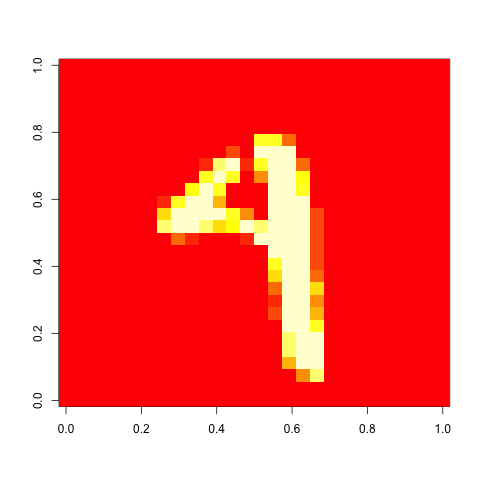
\includegraphics[scale = .25]{../Images/740.png}\caption{Case 740: Predict - 9, True - 4.}\label{fig:taba}\end{subfigure}\\
\newline
\begin{subfigure}{0.3\textwidth}\centering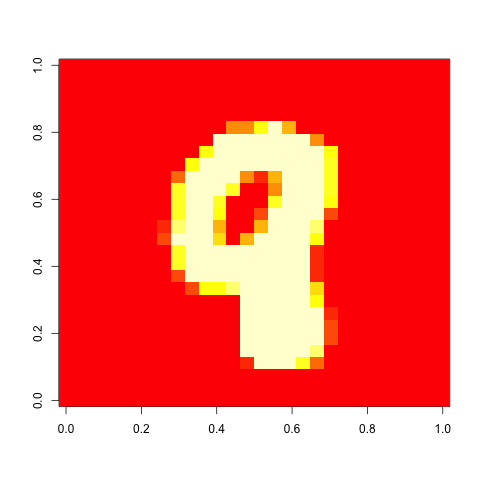
\includegraphics[scale = .25]{../Images/947.png}\caption{Case 947: Predict - 9, True - 8.}\label{fig:taba}\end{subfigure}&
\begin{subfigure}{0.3\textwidth}\centering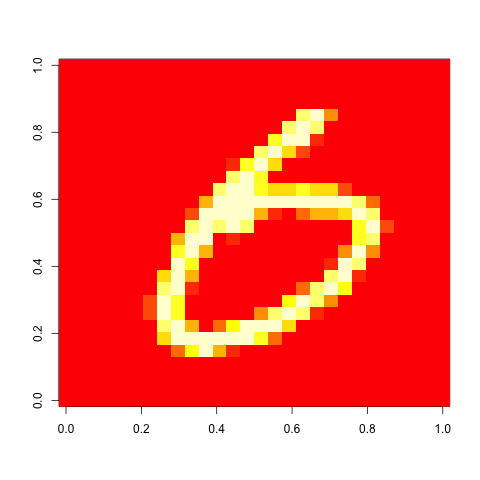
\includegraphics[scale = .25]{../Images/965.png}\caption{Case 965: Predict - 0, True - 6.}\label{fig:taba}\end{subfigure}&
your spot
\end{tabular}
\end{table}


\section{Real World Applications}

While being able to classify numbers provided by test set is cool, its not exactly applicable to the real world. Thus, we found a way to turn an image into .csv format so that it can be predicted by our various models. For the image classification, we used knn. LDA had too big of an error, QDA can not be used unless we have more observations than predictors and random foresting is just incompatible with our data.\\\\
The first step was drawing our data, which we used MSPaint to do. There were small errors when we read the file into R and then scaled it, since if we started with a small image there would be virtually no grayscaling. We found that using a 560x560 pixel image with a brush size of about 40 pixels was optimal for sizing.\\\\
The next problem was turning the data into a format where knn could be run on it. We read the image into R and obtained all the data for each pixel. However, these values were in a 28x28 data frame rather than a vector. Separating out the matrix into a length 784 vector, we were able to run our knn model on the inputted data.

\section{Conclusion}
For LDA, our results of 25\% test error is quite decent for our methods. The main roadblock to LDA was complexity: matrix inversion, which is at the core of LDA, is a computationally expensive routine, so we were forced to use a smaller dataset than possible. Even then, the training phase was sluggish. However, the test phase was instantaneous, in contrast to KNN, but at the cost of a slightly lowered accuracy. \\\\
For QDA, our results were similar to LDA, but all our errors were lower. The training error of 3\% is almost on par with that of KNN, and the test error does not lag behind by much more at 10\%. The major downside to using QDA was that it required a large number of observations, which took more time for R to process.\\\\
For KNN, the findings were essentially opposites of LDA. Our test error was uncannily accurate, with a mere 3\% error rate, and this method requires no training phase. However, its drawback was an extremely sluggish test speed. Of course, reducing the training size could have sped it it up at the cost of accuracy, harkening back to the classic speed-performance tradeoff. \\\\
For random forests, we arrived at the conclusion that this method is simply ineffective for dealing with our task. Since classifying images involves so many predictors, the tree that the algorithm arrives at is cluttered and nonsensical. Our test error was 90\%, no better than a random guess, despite a training error of 54\%. 
\end{document}
















